\section{Arquitectura del Sistema}
\label{sec:arquitectura}

La arquitectura del sistema se organiza en módulos independientes que separan el entorno de simulación, la generación de acciones, la extracción de características, la evaluación de estados y los métodos de aprendizaje. Esta separación permite comparar TD(0) y el Método de Entropía Cruzada sobre una misma función de valor.

\begin{figure}[H]
\centering
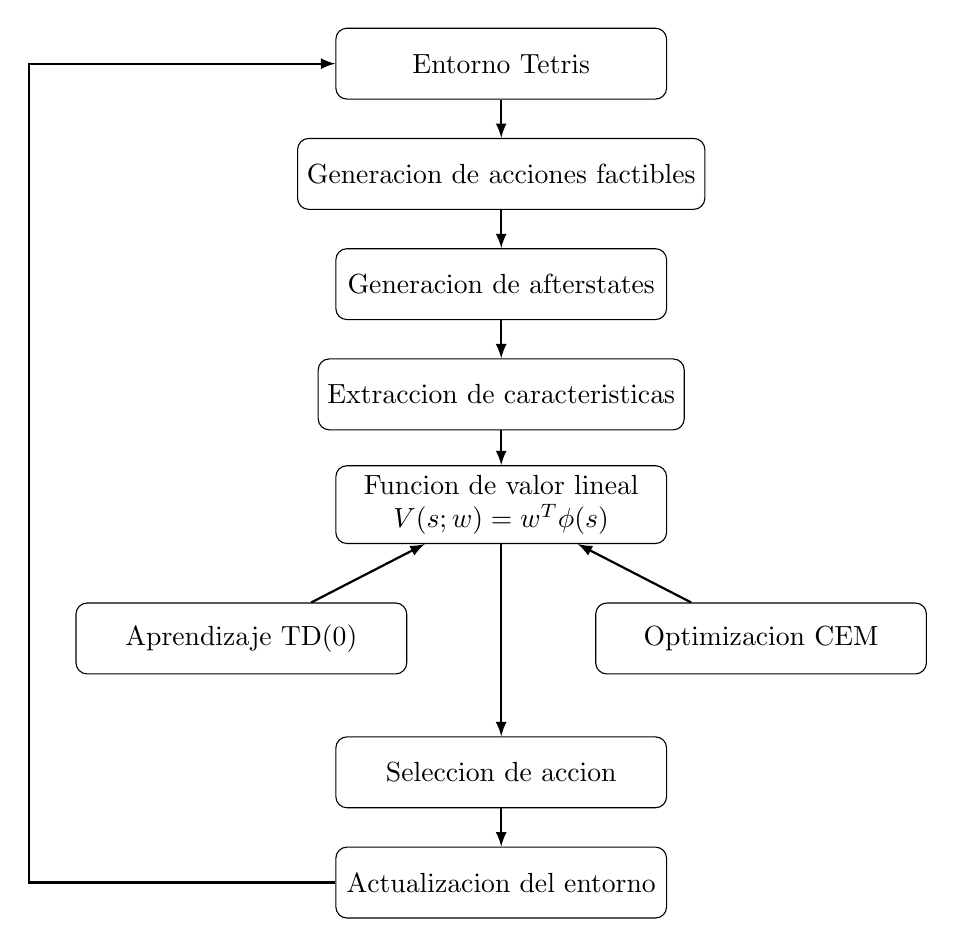
\begin{tikzpicture}[
    block/.style={
        rectangle,
        draw,
        rounded corners,
        align=center,
        minimum width=4.2cm,
        minimum height=0.9cm
    },
    arrow/.style={
        -latex,
        thick
    }
]

\node[block] (env) at (0,0) {Entorno Tetris};
\node[block] (actions) at (0,-1.4) {Generacion de acciones factibles};
\node[block] (after) at (0,-2.8) {Generacion de afterstates};
\node[block] (features) at (0,-4.2) {Extraccion de caracteristicas};
\node[block] (value) at (0,-5.6) {Funcion de valor lineal\\$V(s;w)=w^{T}\phi(s)$};

\node[block] (td) at (-3.3,-7.3) {Aprendizaje TD(0)};
\node[block] (cem) at (3.3,-7.3) {Optimizacion CEM};

\node[block] (policy) at (0,-9.0) {Seleccion de accion};
\node[block] (update) at (0,-10.4) {Actualizacion del entorno};

\draw[arrow] (env) -- (actions);
\draw[arrow] (actions) -- (after);
\draw[arrow] (after) -- (features);
\draw[arrow] (features) -- (value);

\draw[arrow] (td) -- (value);
\draw[arrow] (cem) -- (value);

\draw[arrow] (value) -- (policy);
\draw[arrow] (policy) -- (update);

\coordinate (retorno) at (-6,0);

\draw[arrow]
(update.west)
-- (retorno |- update.west)
-- (retorno)
-- (env.west);

\end{tikzpicture}
\caption{Arquitectura general del agente inteligente para Tetris.}
\label{fig:arquitectura}
\end{figure}

El flujo inicia con el entorno de Tetris, que proporciona el tablero actual y la pieza activa. A partir de este estado se generan las acciones factibles, definidas por una rotación y una columna de colocación. Cada acción produce un tablero resultante o \emph{afterstate}, que luego se transforma en un vector de características.

Los métodos TD(0) y CEM buscan obtener un vector de pesos adecuado para la función de valor. TD(0) actualiza los pesos de forma incremental durante la interacción con el entorno, mientras que CEM realiza una búsqueda poblacional sobre posibles vectores de pesos.